

\chapter{Metodologia}
\label{chapter:metodolia}




\section{Sistema de Teste}


Fazer uma pequena introdução.

Para efetuar o treinamento da rede foram usados os dados providenciados pela Renault Cacia.
	Cada caixa de velocidades é testada pela Renault em uma das suas linhas testagem. De forma simplificada, o teste consiste em fazer o engrenamento e a passagem de cada uma das mudanças de forma decrescente começando pela mudança mais alta (6ª) e terminando na marcha-atrás. Quando uma mudança está engrenada, a caixa é sujeita a uma certa rotação e binário e são feitas as medições correspondentes às métricas referidas na Análise Vibratória \ref{Analise Vibratória}. Após isto, é feita a passagem e o engrenamento da próxima mudança. Durante a passagem da mudança, ou seja, a manipulação do comandos por parte do colaborador, são feitas as medições das métricas relativamente à passagem de mudança * falta adicionar esta parte no estado de arte *. Após o teste estar concluído, a caixa pode ter uma das 3 seguintes classificações: 
\begin{itemize}
\item \textbf{caixa  boa}, nenhuma das métricas passou os limites estabelecidos por análise estatística pela Renault e o colaborador validou a caixa, não tendo pressentido nenhuma anomalia.
\item \textbf{caixa com defeito}, uma das métricas passou os limites estabelecidos por análise estatística pela Renault, ou o colaborador pressentiu uma anomalia com a caixa.
\item \textbf{teste não conclusivo}, o teste não terminou ou foi interrompido pelo colaborador devido ao não cumprimento de condições de teste. Exemplo: a caixa por ser nova, apresenta algum resíduo de fabrico (ex. limalha) entre os dentes das engrenagens, no qual irá se desintegrar após a caixa entrar em rodagem algumas vezes. 
\end{itemize}

A informação relativamente ao teste de uma caixa de velocidade está armazenada num ficheiro. A figura \ref{ensaio} demonstra parte de um ensaio, neste caso só contém a informação relativa à 6 velocidade que é a primeira a ser testada.


\begin{figure}[H]
\centering
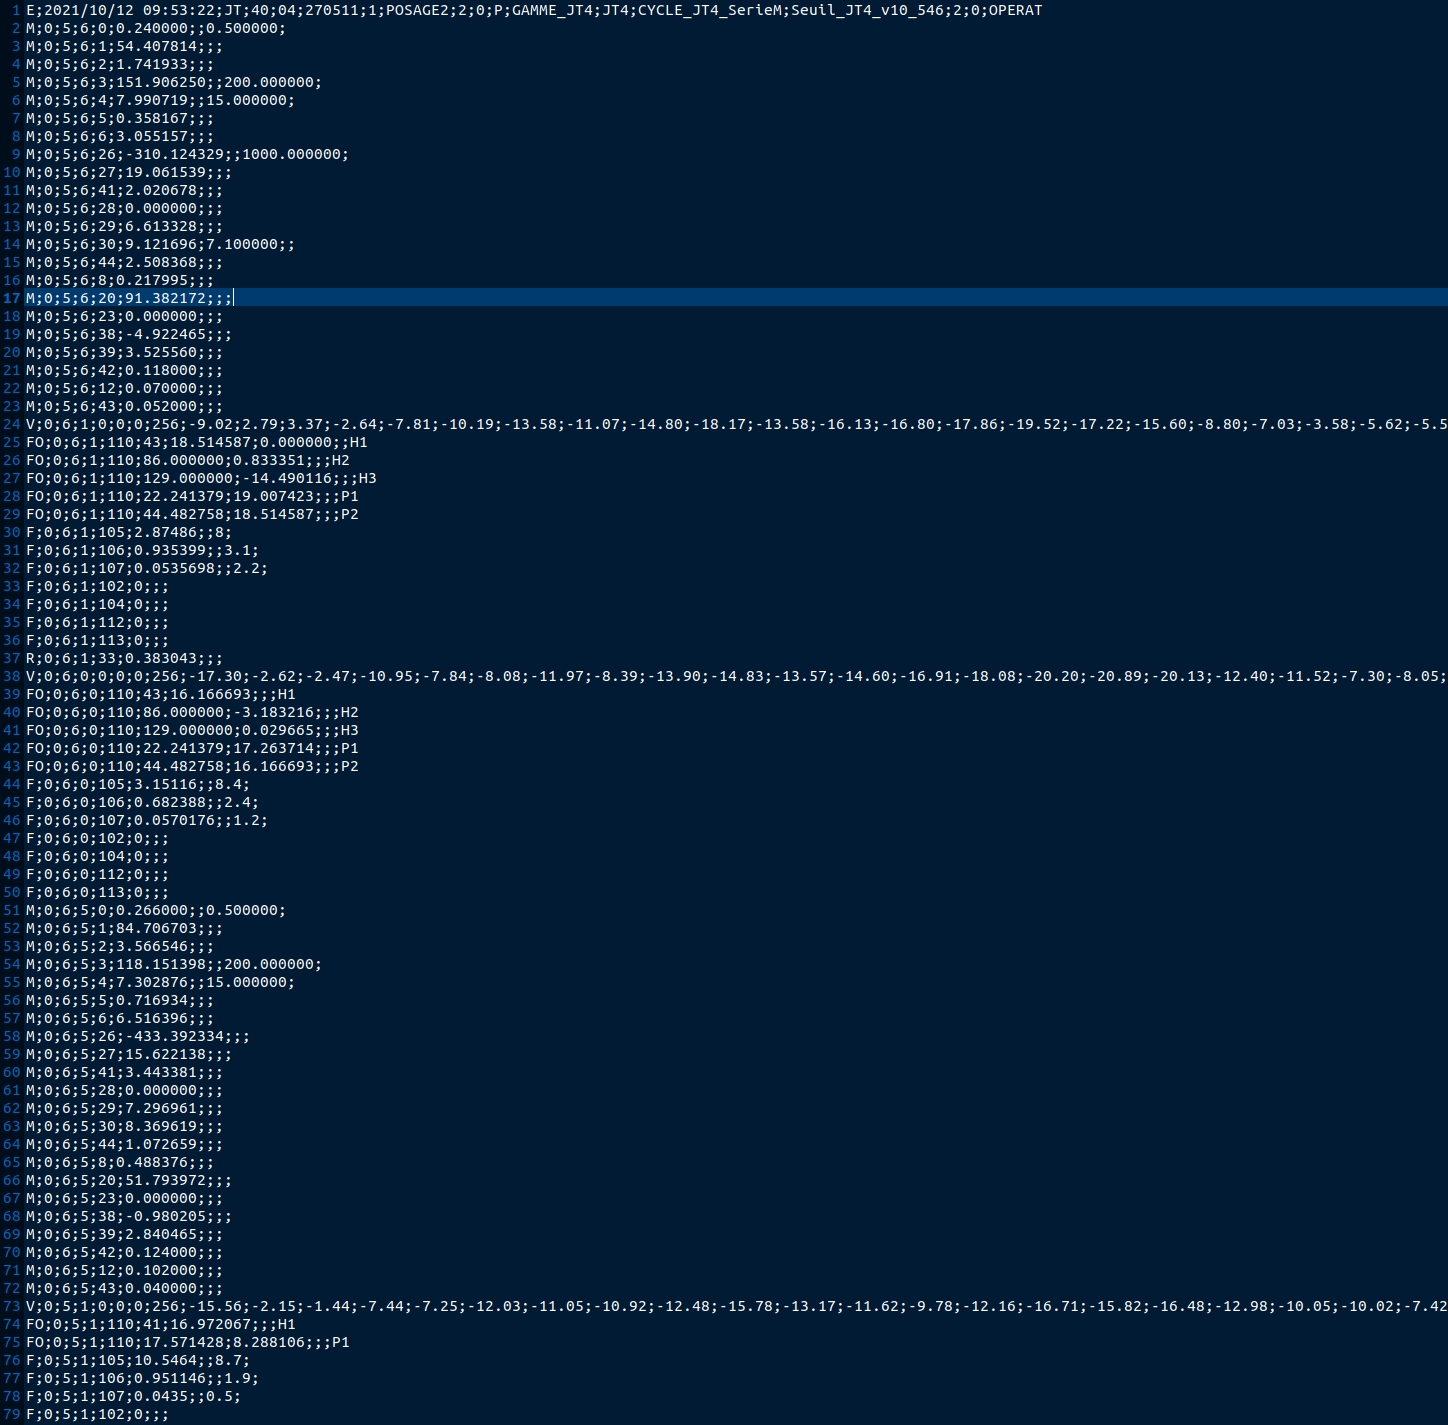
\includegraphics[scale=0.3]{figs/ensaio}
\caption{Parte de um ficheiro correspondente a um ensaio.}\label{ensaio}
\end{figure}









